\documentclass[12pt]{article}
\usepackage[english]{babel}
\usepackage[utf8x]{inputenc}
\usepackage{amsmath}
\usepackage{graphicx}
\usepackage[colorinlistoftodos]{todonotes}
\usepackage[margin=1in]{geometry}

\begin{document}
	
	\begin{titlepage}
		\newcommand{\HRule}{\noindent\rule{6.5in}{1pt}} % Defines a new command for the horizontal lines, change thickness here
		
		\centering
		
		\textsc{\Large Intro to Artificial Intelligence}\\[.75cm]
		
		\noindent\rule{6.5in}{1.5pt}\\[.75cm]
		{ \huge \bfseries Assignment 1}\\[.4cm]
		{ \large \bfseries Fast Trajectory Planning}\\[.2cm]
		\noindent\rule{6.5in}{1.5pt}\\[1cm]
		
		
		\begin{minipage}{0.4\textwidth}
			\begin{flushleft} \large
				\emph{Authors:}\\
				Brian \textsc{Lin} \\
				Samuel \textsc{Yang}
			\end{flushleft}
		\end{minipage}
		~
		\begin{minipage}{0.4\textwidth}
			\begin{flushright} \large
				\emph{Supervisor:} \\
				Dr. Abdeslam  \textsc{Boularias} % Supervisor's Name
			\end{flushright}
		\end{minipage}\\[2cm]

		
\includegraphics[width=200pt,height=200pt]{RutgersLogo.png}\\[1.5cm]
		\textsc{\Large Rutgers State University of New Jersey}\\[1cm]
		{\large \today}\\[2cm]
		
		\vfill % Fill the rest of the page with whitespace
		
	\end{titlepage}
	
	\twocolumn
	
	\section*{Introduction}
	
	This assignment requires the students to implement multiple variants of A* algorithms and analyze the performances of these variants.  The scenario given is as follows, an agent in a gridworld has to move from its current cell to the given cell of a non-moving target, where the gridworld is not fully known. The various cells of the world are either blocked or unblocked, with the dimensions of the gridworld being 101 by 101 cells.  There aere 5 variants of the A* algorithm that are implemented:
	\begin{itemize}
		\item Repeated Forward A* (RFAS)
		\item RFAS with high g-score tiebreaker
		\item RFAS with low g-score tiebreaker
		\item Repeated Backward A* (RBAS)
		\item Adaptive A*
	\end{itemize}   
	RFAS calculates the A* search and then has the agent move one step closer, exploring the neighbors surrounding that cell, and then repeats until the agent reaches the target.  The next two variants simply enforce tie-breaking restrictions on the RFAS search, with cells that have the same f-score being tie-broken by the higher g-score or the lower g-score respectively.  RBAS is similar to the RFAS algorithm, but rather than running the A* search from the agent cell to the target, the A* is computed from the target to the agent cell.  Adaptive A* passes heuristic values into future iterations of A* to reduce computational costs.  All relevant information for this project can be found here: \\ https://github.com/samuel-yang/cs440/tree/master/A1 \\
	This project was coded in Python, and utilizes the pygame package to help display and create an interface for users.  The relevant file for user interaction is pathFinding.py
	
	\section*{Part 1 - Understanding the Methods}
	
	\subsection*{A) - East vs North}
		\begin{figure}[!htb]
			\centering
			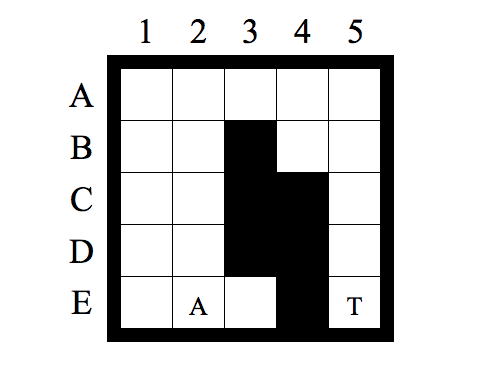
\includegraphics[width=.5\textwidth]{Figure8.png}
			\caption{\label{Figure 8: }Second Example Search Problem}
		\end{figure}
	The agent in the figure above begins it's pathfinding without knowledge of which cells are blocked.  From the perspective of being able to fully observe the maze,
	it appears clear that the best path for the agent is to move north to go around the obstacle.  However, under the initial assumption that all cells are unblocked
	the shortest path from the current cell to the target is to move towards the east, as it has a direct path to the target cell.  Only once the agent has moved to
	the cell to the east, will it observe the blocked cells that do not allow it to use that path and force the agent to find a new path to the target.
	
	\subsection*{B) - Proving Completeness}
	
		Proving the completeness of an A* search algorithm can be observed by first simplifying the search algorithm.  Let the following variables be defined as: 
		\begin{itemize}
			\item g is a graph
			\item S is the start vertex
			\item G is the goal vertex
			\item Q is a list of partial paths in g
		\end{itemize}
		Given the above variables, a modified version of the search algorithm's pseudo code can be found below.
		\begin{enumerate}
			\item Initialize Q with path(s)\\
			set Visited = ()
			\item If Q is empty, return fail\\
			Else pick some partial path N from Q
			\item \textit{// If head(N) = G, return N \\ (This is where the algorithm would normally exit)}
			\item Else
			\begin{enumerate}
				\item Remove N from Q
				\item Find neighbors of head(N) not in visited\\
				Create one-step extension of partial paths from N to child
				\item Add to Q all new paths
				\item Add children of head(N) to visited
				\item Go to step 2
			\end{enumerate}
		\end{enumerate}
	
		From the pseudo code, the following true statements can be observed:
		\begin{itemize}
			\item A path removed from Q is not placed back into Q.
			\item If a vertex v is reachable from S, it will be placed into the visited set in a finite number of steps.
			\item The modified pseudo code will place G into visited if it is reachable.
		\end{itemize}
		During the unmodified search algorithm, the two termination conditions are if there are no more vertices to be visited, or if the goal vertex G is found.  Therefore, the search algorithm is guaranteed to find a solution if one exists.  
		The bounded limit of the number of moves until the agent reaches the target or discovers can be shown to be the unblocked number of cells squared.  The worst case scenario would be if every cell in the gridworld was unblocked, and if the A* search started at every unblocked cell in the gridworld, and the agent visits every other unblocked cell from each initial start position.  By visiting every single cell in the gridworld, the goal is guaranteed to be found and reached.  Or if no goal exists in the gridworld, at the upper limit will be at most the unblocked cell squared.    
	\section*{Part 2 - The Effects of Ties}
		\begin{figure}[!htb]
			\centering
			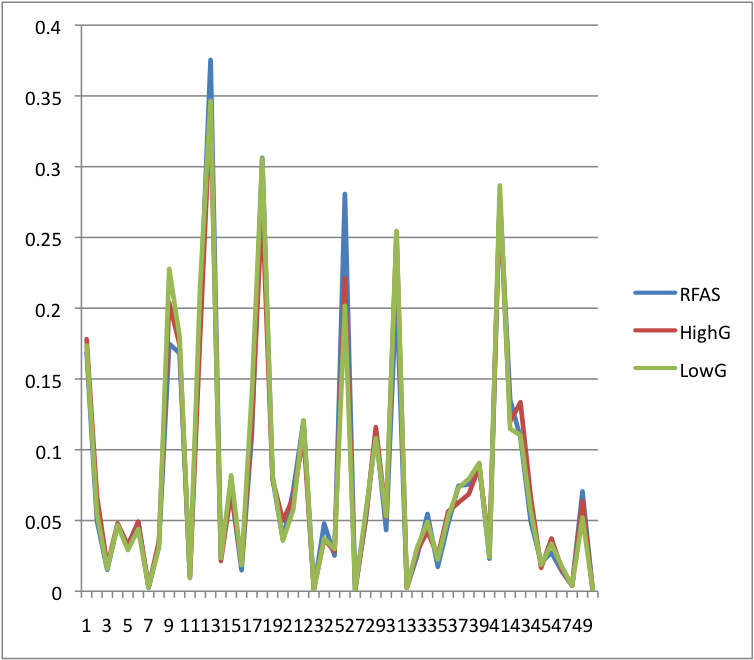
\includegraphics[width=.5\textwidth]{rfas_high_low.png}
			\caption{Effect of g-score based tie-breaking}
		\end{figure}
		The figure above compares the total runtime using 3 different Repeated Forward A* (RFAS) algorithms over 50 test cases. The blue line in the line graph represents the basic RFAS algorithm.  The red line builds on the RFAS by breaking ties between states with the same smallest f-value by choosing the state with the higher g-score.  The green line similarly impacts RFAS by adding in a tiebreaker but instead chooses the state with the lower g-score value.  The data plotted in the figure can be observed in Table 1.  Comparing the total compute times reveals that generally, RFAS implemented with some form of tiebreaker outperformed basic RFAS.  To examine the differences and impact between using based a high g-score or a low g-score on the efficiency of the algorithm, examine Figure 3 and the computational times in Table 1.  
		\begin{figure}[!htb]
			\centering
			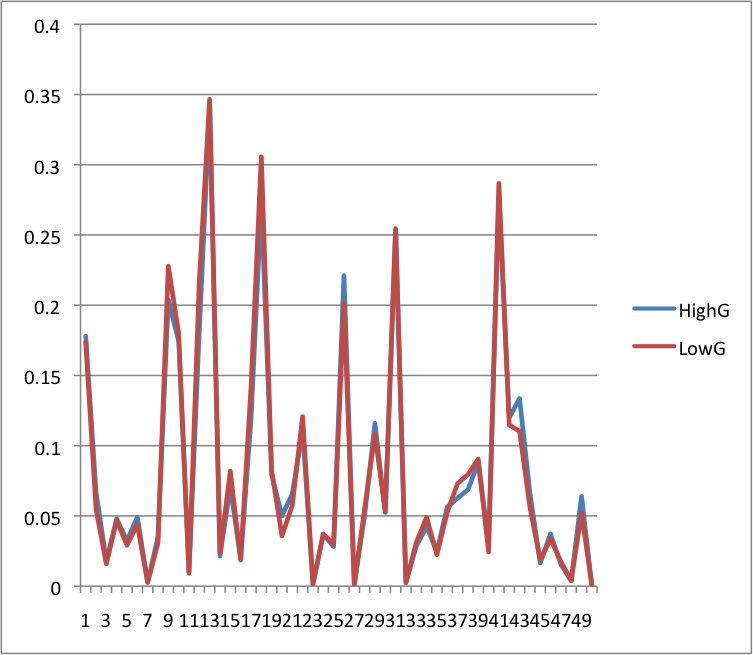
\includegraphics[width=.5\textwidth]{low_high.png}
			\caption{Comparing tie-breaking based on higher g-scores vs lower g-scores}
		\end{figure}
		It is observed that for the majority of test cases, the computational time difference between tiebreakers emphasizing a higher g-score and those that chose a lower g-score were rather small.  However, there is an overall trend of the higher g-score value actually outperforming the lower g-score value that was more observable when the algorithm and the paths were displayed.  To understand the increase in speed and efficiency of the algorithm, recall that the f-score value is a sum of the g-score and the heuristic cost for each cell.  Cells with the same f-score, but having a lower g-score will therefore have a higher heuristic cost, meaning a higher estimate of the moves needed to reach the goal.  Cells with a higher g-score would have a lower heuristic cost and ultimately provide a better path towards the goal cell.  By choosing the higher g-score as a tiebreaker, the agent continues to move towards the target cell while reducing the future distance that would need to be traversed.  
	\section*{Part 3 - Forward vs Backward}
		\begin{figure}[!htb]
			\centering
			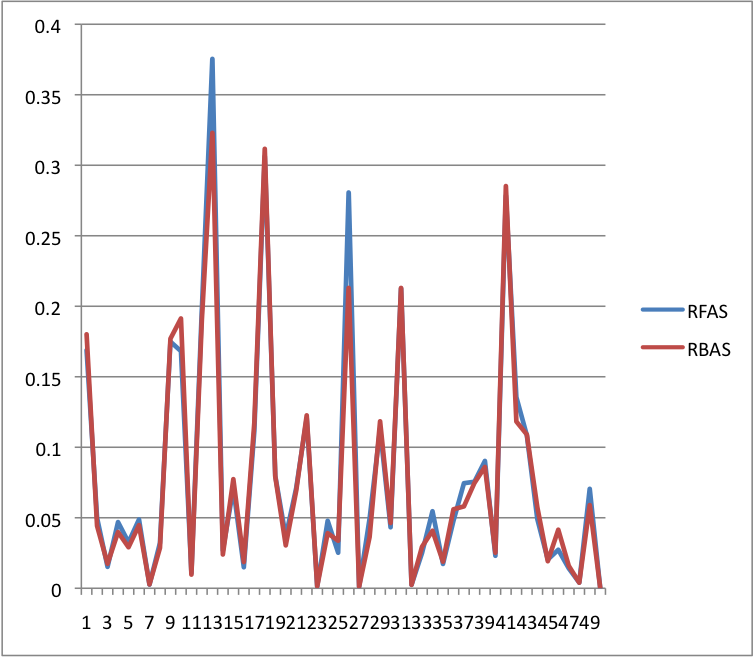
\includegraphics[width=.5\textwidth]{foward_backward.png}
			\caption{Repeated Forward A* vs Repeated Backward A*}
		\end{figure}
		The data represented in the line graph above indicates that again, computational times were incredibly similar.  This time, the comparisons are between Repeated Forward A*, performing the algorithm from the agent cell to the target cell, and Repeated Backward A* (RBAS), having the algorithm traverse the maze from the target cell to the agent.  Examining the data more thoroughly, and observing the displayed output for both instances, it begins to become possible to identify when each algorithm would outperform the other.     
		\onecolumn
		\begin{figure}[!htb]
			\centering
			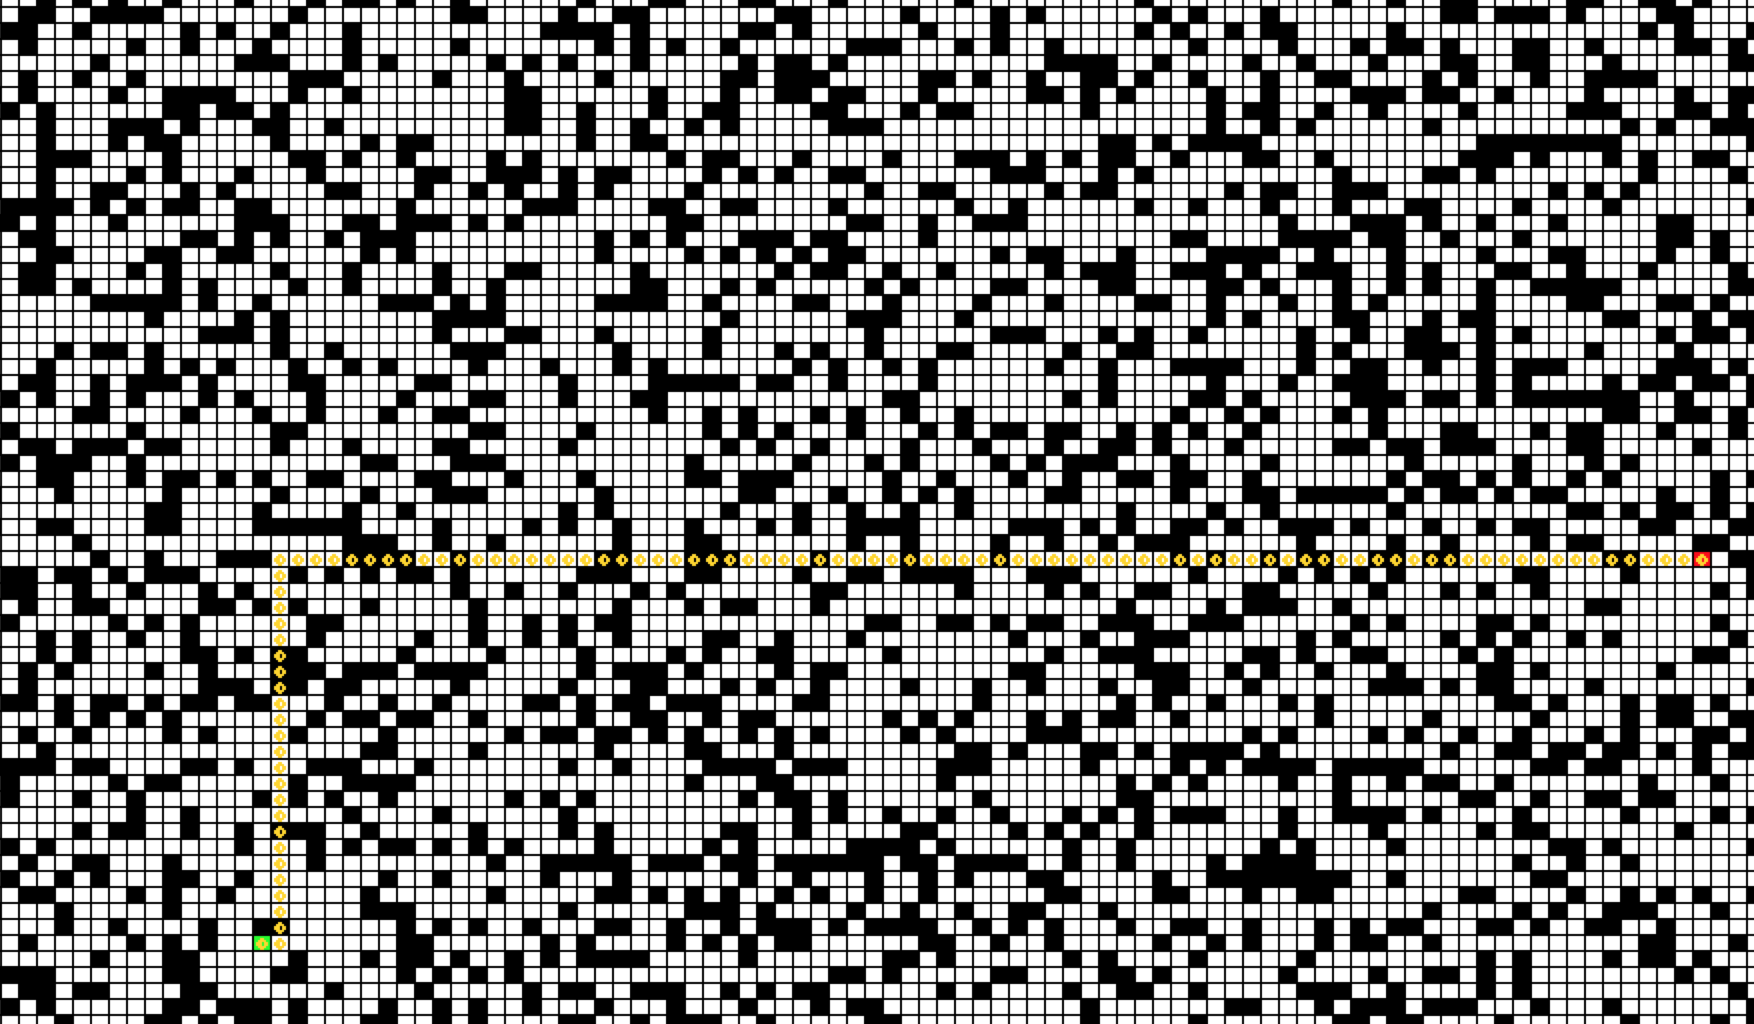
\includegraphics[width=1\textwidth]{test26.png}
			\caption{Test Case 26}
		\end{figure}{1cm}
		In the maze above, the agent cell encounters a heavily blocked off area along its prepared path soon after leaving the initial starting position.  The shape of the blocked cells, rough resembles a wedge, where the agent will move towards the cells at the end of the funnel, as they will have the lowest f-score, but will eventually have to choose a different route as it discovers that there is no viable path through that area.  In this instance, the RBAS algorithm outperformed the RFAS algorithm because when it encounters the blocked off cells that form this trap, it chooses a path that navigates around this obstacle, rather than first exploring it.
		
		In other situations, RFAS is revealed to be the more efficient algorithm than RBAS.  In Figure 6: Test Case 10, found below, one such example can be observed. This time, the target cell has a wedge-like formation of blocked cells that funnels the target cell into more blocked cells until the path would be deemed no longer viable and an alternative one would have to be taken.  
		\twocolumn
		\begin{figure}[!htb]
			\centering
			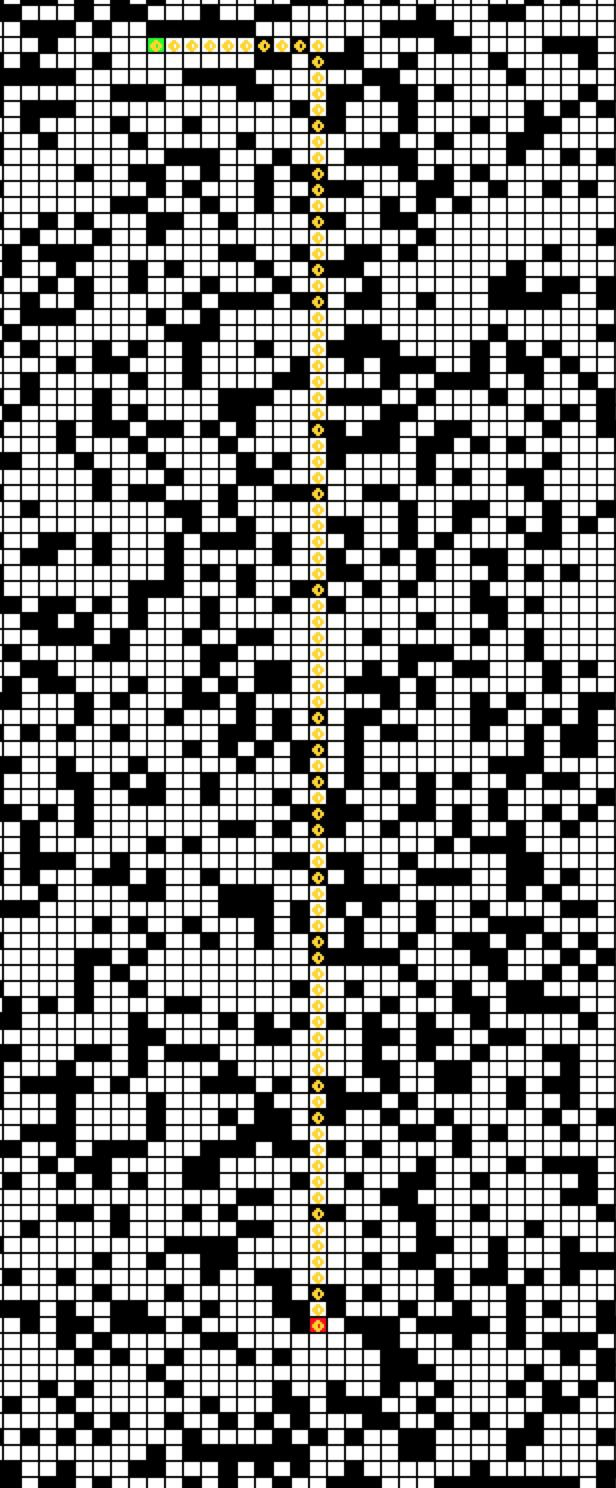
\includegraphics[width=.4\textwidth]{test10.png}
			\caption{Test Case 10}
		\end{figure}  
	
	\section*{Part 4 - Proving Heuristics in the Adaptive A*}
	
		A consistent heuristic function is one where the estimate of a cell will always be less than or equal to the sum of the cost to reach a neighboring cell and the estimated distance from the neighboring cell to the goal.  In other words, the triangle inequality must hold, meaning that the heuristic function must underestimate the actual path cost to the goal.\\
		\\$h(cell)$ $\leq$ $step(neighbor)$ $+$ $h(neighbor)$\\ \\
		This can be proven by understanding what the Manhattan distance represents.  The Manhattan distance is the shortest path to the goal because it is a straight line distance calculation from the given cell to the goal cell.  Any step that is taken will force the path length to increase because it will be deviating from the straight line. 
		
		Adaptive A* also utilizes a consistent heuristic function for all of its estimations of path cost.  Each cell has 4 neighbors that can be visited.  One of the neighbors will be along the original path that was calculated by the previous iteration of adaptive A*, meaning that the actual path cost will be the heuristic cost if the path continues.  One neighbor will move in a direction closer to the goal, however due to the nature of the A* algorithm and the previously addressed consistency of normal A*, this move will not reduce overall path length as it will simply represent a reordering of the movements towards the goal.  Finally, both other legal movements would move the agent further from the goal, meaning that the step cost and the new heuristic cost would be greater than the $h_{new}(s)$ value of the cell.  
		
	\section*{Part 5 - Heuristics in the Adaptive A*}
		\begin{figure}[!htb]
			\centering
			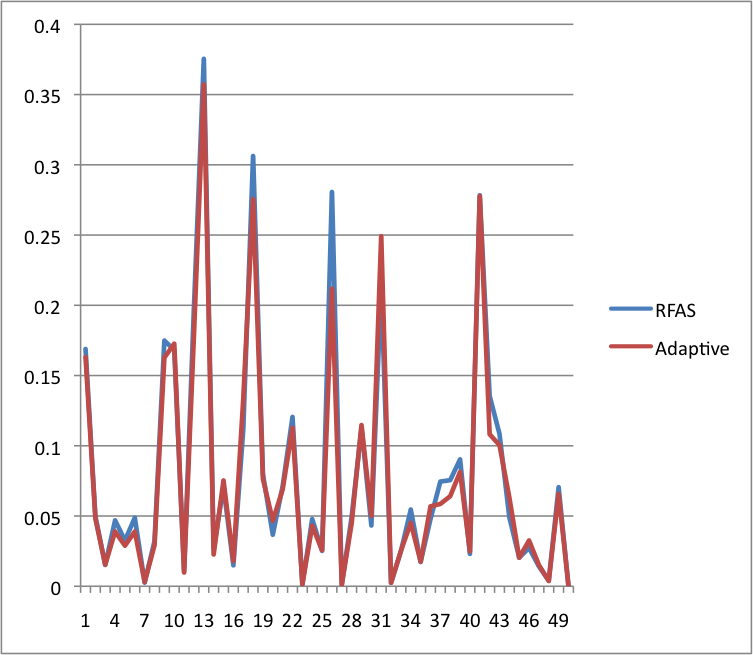
\includegraphics[width=.5\textwidth]{foward_adaptive.png}
			\caption{Comparing RFAS vs Adaptive A*}
		\end{figure}
		The comparison of RFAS and Adaptive A* proved to have the most significant differences in computational times, revealing the observable increase in efficiency that Adaptive A* provides to the algorithm.  During the examination of the various test cases, both algorithms started the initial repetitions at a similar speed.  The speedup became evident as more and more repetitions of A* were computed, as the agent moved away from the initial starting position.  This correlates to the anticipated behavior of Adaptive A* as the implementation of this algorithm means that future A* searches do not have to spend time computing the heuristic costs of previously expanded cells.  Rather, cells that had been expanded in previous iterations would have their heuristics be passed into the current search to reduce the overall computational time.  As the agent moved closer to the target cell, the computational time continued to decrease in comparison to the RFAS.  In all instances where the recorded time of RFAS was faster than the Adaptive A*, the difference was negligible enough that other factors such as processor consistency could account for the time differences.  
	\section*{Part 6 - Memory Issues}
	
	The current implementation is fairly memory efficient in its structure. The main sinks in memory are the openlist and closed list which can be difficult to reduce. The heuristic is already calculated dynamically so we cannot reduce that further.
	
	There are a few ways we could reduce the memory usage of our implementation, but they do require tradeoffs. One way is to use a bloom filter for the closed list, which can basically store all our data in an array of fixed size rather than a set which has store each cell.  By having multiple hash functions on each cell as verification, it provides an easy and efficient way to look up whether a cell has already been expanded. The tradeoff is that it is randomized algorithm that can produce false positives. The amount of storage dedicated to the filter array corresponds to the probability of false positives and can depend on the usage case. Additionally, we could implement a depth checker which is based on the Simplified Bounded A*, which stops the A* search after a certain depth has been reached due to memory restrictions. This will cap the amount of memory the A* search utilizes by a fixed amount but will only be able to find an optimal solution if the solution exists within the memory bounds. This is an extreme case where we may value memory over finding the optimal path.
	
	The best way to optimize memory would be to have the memory pointer be only 2 bits. There are 4 possible states we can use with 2 bits (00 01 10 11) and each could represent a direction from where the child cell came from. In python, a pointer can take up to as much as 24 bytes, this would drastically reduce the memory needed.
	
	For this implementation of A*, we have the 2D array of ints, the closed set, the open set, a g-score, an f-score, and the tree dictionary that keeps track of each cell’s parent. Worst case space complexity would be if every single cell was expanded and has a parent(pointer), a g-score(int), f-score(int), and stored in the closed set(int). Let’s say an int is 4 bytes and a pointer to a parent is 2 bits. That mean each cell requires $16 bytes + 2 bits = 16.25$. Thus a 1001 x 1001 has 1002001 cells, which is $1002001 * 16.25 = 16.3MB$ in the worst case. For 4MB, you would be able hold $4,194,304 / 16.25 = 258,000k cells$ or about a 508 x 508 grid. 
	
	\onecolumn
	\section*{Recorded Data}
		\begin{table}[!htb]
			\centering
			\begin{tabular}{|c|c|c|c|c|c|}
				Testcase & R.Foward A* &  RFAS HighG & RFAS LowG & R.Backward A* & Adaptive A*\\\hline
				1&0.16886&0.17805&0.17369&0.1801&0.16311\\
				2&0.04992&0.06725&0.05501&0.04421&0.04815\\
				3&0.0152&0.01764&0.01579&0.01735&0.01532\\
				4&0.04691&0.048&0.04682&0.03984&0.03901\\
				5&0.03259&0.0322&0.02912&0.02909&0.02887\\
				6&0.04877&0.04917&0.04396&0.04474&0.03894\\
				7&0.00258&0.00278&0.00273&0.00274&0.0031\\
				8&0.03216&0.03524&0.03074&0.02859&0.02917\\
				9&0.17487&0.20381&0.22777&0.17702&0.1627\\
				10&0.16817&0.17427&0.18004&0.19133&0.17266\\
				11&0.01085&0.0102&0.00923&0.00969&0.0098\\
				12&0.19812&0.18156&0.21727&0.19082&0.17869\\
				13&0.37543&0.34151&0.34659&0.32296&0.3571\\
				14&0.027&0.02141&0.02349&0.02396&0.02264\\
				15&0.07082&0.07063&0.08186&0.07736&0.07528\\
				16&0.01491&0.01939&0.01864&0.01861&0.01785\\
				17&0.11103&0.11815&0.14064&0.11699&0.1328\\
				18&0.30625&0.27258&0.30568&0.31164&0.27548\\
				19&0.07971&0.07944&0.08235&0.07921&0.0765\\
				20&0.03667&0.04993&0.03576&0.03042&0.04663\\
				21&0.07115&0.06586&0.05749&0.06926&0.06892\\
				22&0.12052&0.11078&0.12065&0.12261&0.11285\\
				23&0.00138&0.00139&0.0014&0.00141&0.00136\\
				24&0.04784&0.037&0.03721&0.03908&0.04306\\
				25&0.02521&0.02815&0.02986&0.0337&0.02562\\
			\end{tabular}
		\end{table}
		\begin{table}[!htb]
			\centering
			\begin{tabular}{|c|c|c|c|c|c|}
				Testcase & R.Foward A* &  RFAS HighG & RFAS LowG & R.Backward A* & Adaptive A*\\\hline
				26&0.28067&0.22102&0.20164&0.213&0.21173\\
				27&0.00112&0.00096&0.00111&0.00118&0.00114\\
				28&0.04938&0.05022&0.05515&0.03637&0.04476\\
				29&0.11286&0.11589&0.1081&0.11839&0.11472\\
				30&0.04326&0.0525&0.05303&0.04632&0.05009\\
				31&0.21258&0.25313&0.25453&0.21298&0.24917\\
				32&0.00248&0.00249&0.00244&0.00244&0.00246\\
				33&0.02496&0.02853&0.03103&0.02944&0.02524\\
				34&0.05461&0.04239&0.04902&0.04079&0.04513\\
				35&0.01725&0.0248&0.02236&0.01885&0.01753\\
				36&0.04785&0.05629&0.0526&0.056&0.05686\\
				37&0.07451&0.06268&0.07305&0.05806&0.0586\\
				38&0.07553&0.06864&0.07941&0.07465&0.06411\\
				39&0.09029&0.08791&0.09055&0.08602&0.08135\\
				40&0.02305&0.0311&0.02434&0.02521&0.0249\\
				41&0.27835&0.27648&0.28678&0.28523&0.27768\\
				42&0.13551&0.11997&0.11477&0.11826&0.1082\\
				43&0.10844&0.13354&0.11034&0.10902&0.10043\\
				44&0.04908&0.06643&0.05641&0.05744&0.06319\\
				45&0.02036&0.01654&0.01862&0.01919&0.02032\\
				46&0.02731&0.03726&0.03352&0.04151&0.03259\\
				47&0.0141&0.01551&0.01756&0.01589&0.01512\\
				48&0.00401&0.00388&0.00393&0.00397&0.00373\\
				49&0.0705&0.06386&0.05215&0.05897&0.06572\\
				50&0.00026&0.00026&0.00039&0.00031&0.00023\\
			
			\end{tabular}
			\caption{\label{tab:widgets}An example table.}
		\end{table}
	\iffalse
		\section{Some \LaTeX{} Examples}
		\label{sec:examples}
		
		\subsection{Sections}
		
		Use section and subsection commands to organize your document. \LaTeX{} handles all the formatting and numbering automatically. Use ref and label commands for cross-references.
		
		\subsection{Comments}
		
		Comments can be added to the margins of the document using the \todo{Here's a comment in the margin!} todo command, as shown in the example on the right. You can also add inline comments too:
		
		\todo[inline, color=green!40]{This is an inline comment.}
		
		\subsection{Tables and Figures}
		
		Use the table and tabular commands for basic tables --- see Table~\ref{tab:widgets}, for example. You can upload a figure (JPEG, PNG or PDF) using the files menu. To include it in your document, use the includegraphics command as in the code for Figure~\ref{fig:frog} below.
		
		% Commands to include a figure:
		%\begin{figure}
		%	\centering
			%\includegraphics[width=0.5\textwidth]{frog.jpg}
		%	\caption{\label{fig:frog}This is a figure caption.}
		%\end{figure}
		
		%\begin{table}
		%%	\begin{tabular}{l|r}
				%Item & Quantity \\\hline
				%Widgets & 42 \\
				%Gadgets & 13
		%	\end{tabular}
		%	\caption{\label{tab:widgets}An example table.}
		%\end{table}
		
		\subsection{Mathematics}
		
		\LaTeX{} is great at typesetting mathematics. Let $X_1, X_2, \ldots, X_n$ be a sequence of independent and identically distributed random variables with $\text{E}[X_i] = \mu$ and $\text{Var}[X_i] = \sigma^2 < \infty$, and let
		$$S_n = \frac{X_1 + X_2 + \cdots + X_n}{n}
		= \frac{1}{n}\sum_{i}^{n} X_i$$
		denote their mean. Then as $n$ approaches infinity, the random variables $\sqrt{n}(S_n - \mu)$ converge in distribution to a normal $\mathcal{N}(0, \sigma^2)$.
		
		\subsection{Lists}
		
		You can make lists with automatic numbering \dots
		
		\begin{enumerate}
			\item Like this,
			\item and like this.
		\end{enumerate}
		\dots or bullet points \dots
		\begin{itemize}
			\item Like this,
			\item and like this.
		\end{itemize}
	\fi
	

\end{document}